\section{\textsc{FlashSigmoid}: Hardware-Aware Implementation}
\label{sec:FlashSigmoidHardwareAwareImplementation}
\begin{figure}[!thbp]
    \centering
    \begin{minipage}{0.45\textwidth}
        \footnotesize
        \centering
        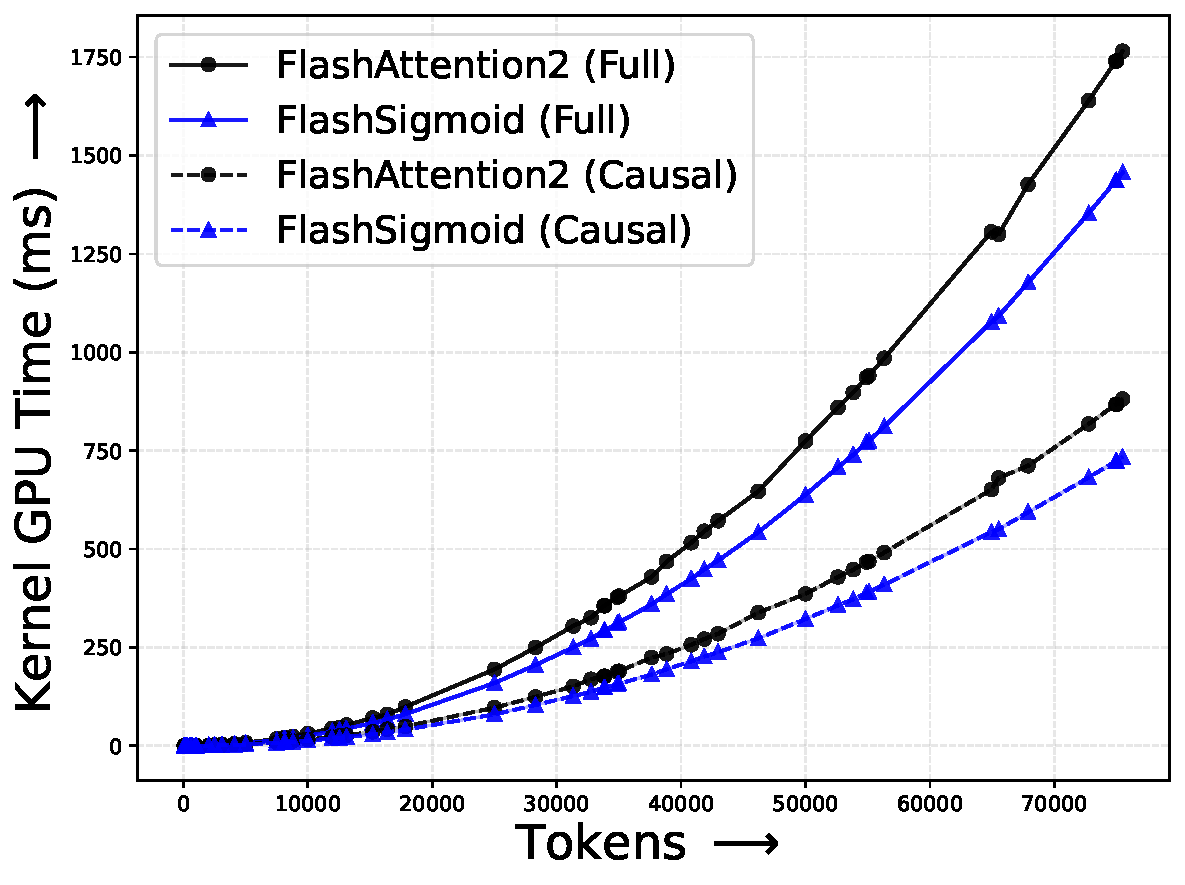
\includegraphics[trim={0 0 0 0}, width=\textwidth]{figures/_flash_figures/final_arxiv/main/H100_noalibi_FWD_Full_17.39_0.07_Causal_18.76_0.06.pdf}
        \captionsetup{justification=centering} 
        \caption*{(a) Inference mode kernels on H100.}
    \end{minipage}
    \hfill
    \begin{minipage}{0.45\textwidth}
        \centering        
        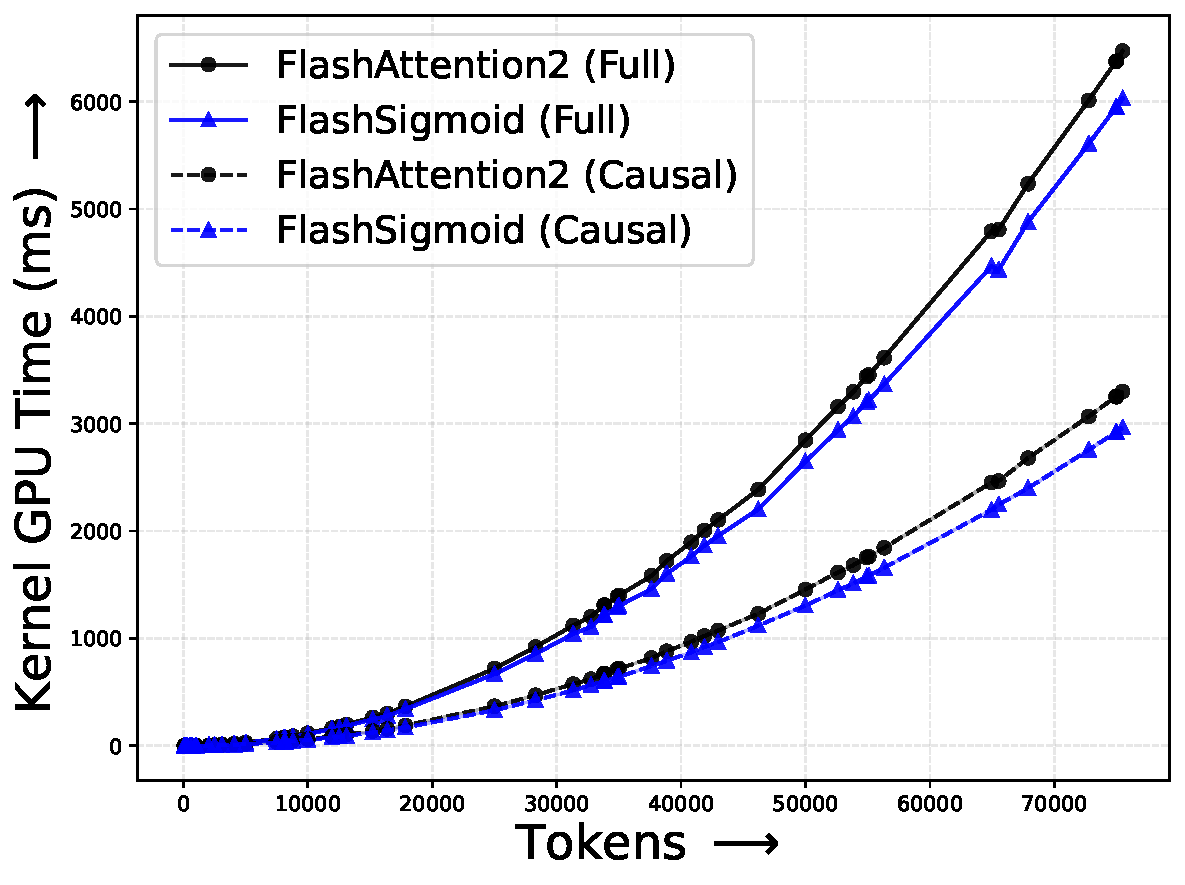
\includegraphics[trim={{0 0 0 0}}, width=\textwidth]{figures/_flash_figures/final_arxiv/main/H100_noalibi_FWDBWD_Full_6.53_0.06_Causal_9.46_0.04.pdf}
        \captionsetup{justification=centering} 
        \caption*{(b) Training mode kernels on H100.}
    \end{minipage}
    \caption{
        Average kernel speed-up for \textsc{FlashSigmoid} over \textsc{FlashAttention2} for sequence lengths 64--78k. Inference is ${17.39}\%$ faster for self-attention and ${18.76}\%$ for causal attention. Training is $6.53\%$ faster for self-attention and $9.46\%$ for causal attention. 
    }
    \label{fig:h100-softmax-sigmoid-main-figure}
    \vspace{-0.2cm}
\end{figure}
Memory speed has not kept pace with recent gains in computation speed~\citep{DBLP:journals/micro/Choquette23,DBLP:conf/isca/JouppiYPPABBBBB17,mlx2023}.
Consequently, attention computations on modern architectures have been IO-bound by memory accesses \citep{DBLP:conf/mlsys/IvanovDB0H21}. 
\textsc{FlashAttention} \citep{DBLP:conf/nips/DaoFERR22} and \textsc{FlashAttention2} \citep{DBLP:journals/corr/abs-2307-08691} address these shortcomings by optimizing GPU memory hierarchy utilization to accelerate attention computations. 
Motivated by the speed boost provided by these approaches, we develop \textsc{FlashSigmoid}, a hardware-aware implementation of $\sigmoidattn$.
Like previous works, \textsc{FlashSigmoid} employs three core ideas:
\paragraph{Tiling: Divide and Conquer Approach to Attention:}\ Similar to \textsc{FlashAttention} and \textsc{FlashAttention2}, \textsc{FlashSigmoid} processes input parts in parallel to compute attention outputs in blocks, efficiently combining partial results to generate the final attention output.
\paragraph{Kernel Fusion:}\ Like \textsc{FlashAttention} and \textsc{FlashAttention2}, \textsc{FlashSigmoid} implements the computational steps of both forward and backward passes of $\sigmoidattn$ as single GPU kernels, minimizing memory accesses and improving memory efficiency by avoiding materialization of intermediate activations on High-Bandwidth Memory (HBM).
\paragraph{Activation Recomputation:}\ The backward pass of sigmoid attention requires the sigmoid activation matrix, which, if materialized on GPU HBM, results in slower implementation and memory inefficiencies. \textsc{FlashSigmoid} addresses this by retaining only query, key, and value tensors for re-computation of the sigmoid activation matrix during the backward pass. Despite increased FLOPs, this approach proves faster in wall-clock time as well as more memory-efficient than the alterantive approach of materializing and retaining the attention matrix.

The forward and backward pass algorithms of \textsc{FlashSigmoid} can be found in~\cref{sec:DetailsOfFlashSigmoidAlgorithm}.
Here, we highlight key differences between \textsc{FlashSigmoid} and \textsc{FlashAttention}/\textsc{FlashAttention2}. 
The point-wise nature of $\sigmoidattn$ results in a faster and more memory-efficient implementation by removing the need to compute the softmax normalization and materialize it to HBM. 
A reduction in the number of kernel dispatches also speeds up \textsc{FlashSigmoid}. 
Further, \textsc{FlashSigmoid} does not require accumulation and tracking of intermediate variables (row-sum and maximum of blocks) in the forward and backward passes which saves computation cost and reduces register pressure. 
We use $\textrm{sigmoid}\left(x\right) = 0.5\cdot\left(1 + \textrm{tanh}\left(0.5\cdot x\right)\right)$ to optimize the sigmoid computation on GPU. 
The speed up in \textsc{FlashSigmoid} compared to \textsc{FlashAttention} arises from optimizing hardware bottlenecks; theoretically, $\sigmoidattn$ is slower than $\softmaxattn$ (\cref{sec:parameter_and_flops}).


To measure the performance improvements of \textsc{FlashSigmoid}, we compare the timings of the kernels in its forward and backward passes against those of \textsc{FlashAttention2}.
The details of this benchmarking on H100 and A100 GPUs can be found in~\cref{sec:PerformanceAnalysisOfFlashSigmoidKernels}.
Measuring GPU computation time, we observe a $17.39\%$ speed-up during inference and a $6.53\%$ speed-up during training for attention over randomly initialized data on H100 GPU (\cref{fig:h100-softmax-sigmoid-main-figure}). 
In practice, these gains may be affected by other bottlenecks, such as movement of tensors between CPU or GPU memory, computations in other layers, and communication overhead in distributed training and inference. 
However, we demonstrate that \textsc{FlashSigmoid} speeds up training by {\textbf{$\sim$4\%} and inference by {\textbf{$\sim$8\%} in a realistic end-to-end setup. 
The details of wall-clock time improvements with~\textsc{FlashSigmoid} are in \cref{sec:SpeedBoostsOfFlashSigmoidInRealisticSettings}.
We also note that practical machine learning workflows are dominated by inference rather than training. 




